\documentclass[tikz,border=10pt]{standalone}
\usepackage{amsmath,amssymb}
\usepackage{tikz}
\usepackage{pgfplots}
\pgfplotsset{compat=1.18}
\usetikzlibrary{arrows.meta,calc,patterns,positioning,shapes,decorations.markings,backgrounds,fit,intersections}
\usepgfplotslibrary{fillbetween}

% Atlas colors
\definecolor{AtlasTeal}{HTML}{5BA4A4}
\definecolor{AtlasTealDark}{HTML}{4A8F8F}
\definecolor{AtlasTealLight}{HTML}{E8F4F4}
\definecolor{AtlasDeep}{HTML}{2C5F5F}
\definecolor{AtlasSage}{HTML}{7BAE7F}
\definecolor{AtlasSageLight}{HTML}{EDF5EE}
\definecolor{AtlasWarm}{HTML}{D4A853}
\definecolor{AtlasWarmLight}{HTML}{FDF6E8}

\begin{document}
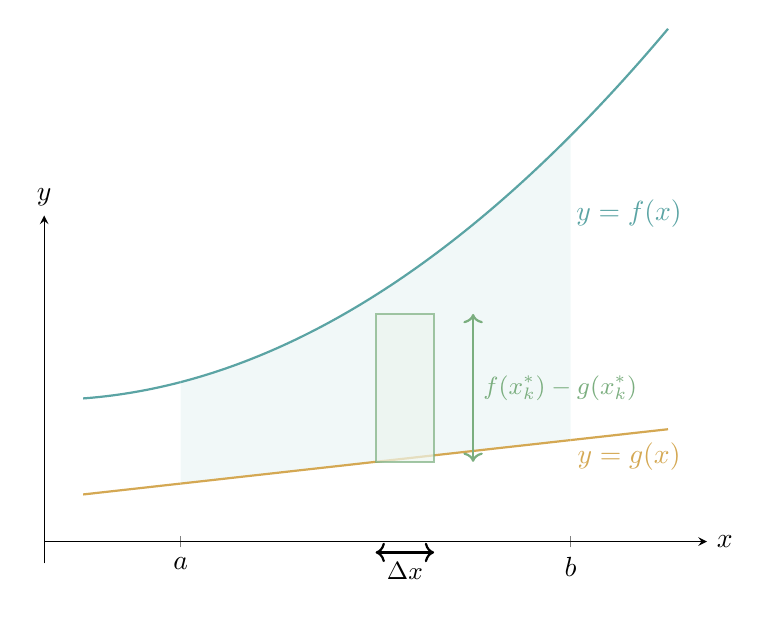
\begin{tikzpicture}
  \begin{axis}[
    width=10cm, height=6cm,
    axis lines=middle,
    xlabel={$x$}, ylabel={$y$},
    xtick={1,3}, xticklabels={$a$,$b$},
    ytick=\empty,
    xmin=0.3, xmax=3.7, ymin=-0.3, ymax=4.5,
    every axis x label/.style={at={(ticklabel* cs:1)}, anchor=west},
    every axis y label/.style={at={(ticklabel* cs:1)}, anchor=south},
    clip=false,
  ]
    % Shaded region
    \addplot[name path=F, AtlasTeal, thick, samples=100, domain=1:3] 
      {0.5*x^2 - 0.3*x + 2};
    \addplot[name path=G, AtlasWarm, thick, samples=100, domain=1:3] 
      {0.3*x + 0.5};
    \addplot[AtlasTealLight, opacity=0.6] fill between[of=F and G];
    
    % Extend curves
    \addplot[AtlasTeal, thick, samples=50, domain=0.5:1] {0.5*x^2 - 0.3*x + 2};
    \addplot[AtlasTeal, thick, samples=50, domain=3:3.5] {0.5*x^2 - 0.3*x + 2};
    \addplot[AtlasWarm, thick, samples=50, domain=0.5:1] {0.3*x + 0.5};
    \addplot[AtlasWarm, thick, samples=50, domain=3:3.5] {0.3*x + 0.5};
    
    % Sample rectangle
    \addplot[AtlasSage, fill=AtlasSageLight, opacity=0.7, thick] 
      coordinates {(2,1.1) (2.3,1.1) (2.3,3.14) (2,3.14)} -- cycle;
    
    % Labels
    \node[above, AtlasTeal] at (axis cs:3.3,4.2) {$y=f(x)$};
    \node[below, AtlasWarm] at (axis cs:3.3,1.5) {$y=g(x)$};
    
    % Height annotation
    \draw[<->, thick, AtlasSage] (axis cs:2.5,1.1) -- 
      node[right, font=\small] {$f(x_k^*)-g(x_k^*)$} (axis cs:2.5,3.14);
    \draw[<->, thick] (axis cs:2,-0.15) -- 
      node[below, font=\small] {$\Delta x$} (axis cs:2.3,-0.15);
  \end{axis}
\end{tikzpicture}
\end{document}
